\section{Empirical study}
This section will be dedicated to the results of the first research question: \textit{What is the current state of the art and what is the performance of these tools?}. 
~\\The tools that have been selected to represent the state of the art have been discussed in both \autoref{chap:background} and \autoref{chap:methodology}. The results will now dive into the second part of the research question, as the performance results from the empirical study executed will be presented below. 

\subsection{Overall results}
\label{subsec:empirical_overall_results}
An aggregate of all the performance scores is shown in \autoref{tab:empirical_results}. All human-aided tools with a maximum of 20 (perfectly accurate) human interactions and all the other non-human interactive tools are used in this aggregate. Then, the performance scores with the highest F1-score for all configurations of a tool are kept per dataset. Precision, recall and the F1-score are shown from left to right per column. The best score for each dataset is marked bold.

\begin{table}[H]
\centering
\caption{|Precision Recall F1| for tool as column \& dataset as row (best scores in bold)}
\label{tab:empirical_results}
\begin{adjustbox}{center}
\begin{tabular}{lllllll}
\toprule
{} & ActiveClean & FAHES & ForbiddenItemSets & KATARA & Raha & dBoost \\
\midrule
 & \textbf{\space\space\space P \space\space\space\space R \space\space\space F1} & \textbf{\space\space\space P \space\space\space\space R \space\space\space F1} & \textbf{\space\space\space P \space\space\space\space R \space\space\space F1} & \textbf{\space\space\space P \space\space\space\space R \space\space\space F1} & \textbf{\space\space\space P \space\space\space\space R \space\space\space F1} & \textbf{\space\space\space P \space\space\space\space R \space\space\space F1} \\
airbnb & 0.15 \textbf{1.00} 0.26 & \textbf{0.54} 0.01 0.02 & 0.13 0.29 0.18 & Other error & 0.42 0.13 0.20 & 0.23 0.38 \textbf{0.28} \\
beers & 0.16 \textbf{1.00} 0.28 & 0.83 0.02 0.04 & 0.34 0.30 0.32 & 0.14 0.26 0.18 & \textbf{0.97} 0.69 \textbf{0.80} & 0.68 0.55 0.61 \\
eeg & 0.04 0.03 0.03 & 0.00 0.00 0.00 & 0.02 0.26 0.04 & 0.00 0.00 0.00 & \textbf{0.56} 0.71 \textbf{0.63} & 0.13 \textbf{1.00} 0.23 \\
flights & 0.30 \textbf{0.98} 0.46 & 0.23 0.01 0.02 & 0.56 0.16 0.24 & 0.09 0.09 0.09 & 0.90 0.83 \textbf{0.86} & \textbf{0.94} 0.59 0.72 \\
hospital & 0.03 0.47 0.05 & 0.02 0.09 0.04 & 0.01 0.06 0.02 & 0.08 0.37 0.13 & \textbf{0.98} \textbf{0.57} \textbf{0.72} & 0.03 0.43 0.06 \\
marketing & 0.25 0.36 0.30 & 0.24 0.01 0.01 & 0.25 0.46 0.33 & 0.21 0.32 0.25 & \textbf{0.50} 0.32 0.39 & 0.34 \textbf{0.67} \textbf{0.45} \\
movie & 0.37 \textbf{1.00} 0.54 & 0.00 0.00 0.00 & 0.31 0.08 0.13 & 0.43 0.43 0.43 & \textbf{0.47} 0.64 \textbf{0.54} & 0.37 \textbf{1.00} 0.54 \\
movies & 0.02 0.00 0.01 & 0.01 0.10 0.02 & 0.01 0.06 0.01 & 0.02 0.16 0.03 & \textbf{0.72} \textbf{0.76} \textbf{0.74} & 0.01 0.09 0.03 \\
rayyan & 0.09 \textbf{1.00} 0.16 & 0.07 0.04 0.05 & Other error & 0.01 0.02 0.01 & \textbf{0.86} 0.84 \textbf{0.85} & 0.22 0.77 0.34 \\
restaurant & 0.01 \textbf{0.83} 0.02 & 0.00 0.00 0.00 & 0.01 0.07 0.01 & 0.00 0.13 0.01 & \textbf{0.14} 0.11 \textbf{0.12} & 0.03 0.03 0.03 \\
restaurants & 0.00 0.00 0.00 & \textbf{0.00} 0.07 \textbf{0.01} & Other error & 0.00 0.22 0.00 & 0.00 \textbf{1.00} 0.00 & 0.00 0.08 0.00 \\
toy & Other error & 0.00 0.00 0.00 & 0.00 0.00 0.00 & 0.21 0.75 0.33 & 0.22 \textbf{1.00} 0.36 & \textbf{0.33} 0.75 \textbf{0.50} \\
university & 0.03 0.09 0.04 & 0.00 0.00 0.00 & Other error & 0.06 0.29 0.10 & \textbf{0.99} 0.91 \textbf{0.95} & 0.32 \textbf{1.00} 0.49 \\
uscensus & 0.02 0.00 0.00 & 0.01 0.18 0.02 & 0.02 0.26 0.04 & 0.00 0.00 0.00 & \textbf{1.00} \textbf{1.00} \textbf{1.00} & 0.41 \textbf{1.00} 0.58 \\
\bottomrule
\end{tabular}
\end{adjustbox}
\end{table}

The results above are also shown as boxplots in \autoref{fig:f1_boxplot} to show a direct overview of the best performing configurations per tool, measured by the F1 score. From the table and figures shown, the conclusion can be drawn that Raha performs best overall for all the tools. Because Raha uses different underlying error detection techniques, it can detect a wide range of errors. In this setup were the error detection task was to detect not only specific errors, but all sorts, the more general methods perform better.
% Non human expert
\\From the non-interactive tools, dBoost performs the best. This might mean that in the majority of datasets used, errors were detectable using rule violations, pattern violations or outliers. 
Besides Raha, the other human interactive tool ActiveClean is the next best tool on average. However, this tool mostly scores best when marking all the values as errors, when the datasets have relatively more errors. Example datasets with low data quality (high percentage of errors) include the datasets movie or flights (see statistics in \autoref{tab:dataset_statistics}). 
The last tools, FAHES, ForbiddenItemSets and KATARA perform worst overall. FAHES is a relatively specific tool, as it mainly tries to find disguised missing values. It could maybe fit in the data cleaning pipeline somewhere where only the missing values need to be detected. ForbiddenItemSets scores a decent average F1-score, as shown in \autoref{fig:f1_boxplot}, but does not cut it against the top 3. It does have higher precision than FAHES and KATARA overall, making it maybe possible to use in an automated fashion, or as a submodule in a composite method like Raha. Lastly, KATARA also performs below average. This is due to the fact that KATARA is highly dependent on the domain the dataset has and the domain given to KATARA as a knowledge base. Apparently, the combination of knowledge base parts was not suited well enough for the test datasets.

\begin{figure}
\centering
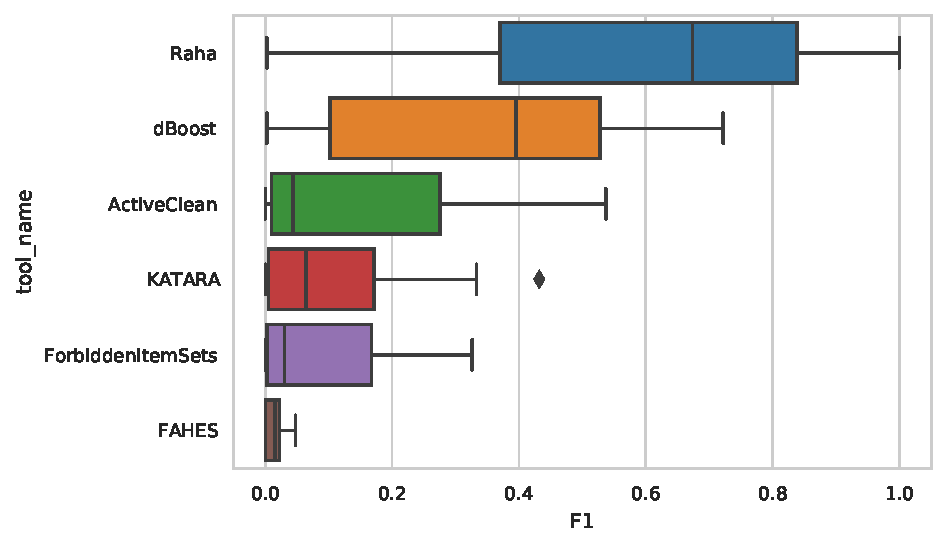
\includegraphics[width=0.9\textwidth]{Figures/RQ1/F1Boxplot.pdf}
\caption{F1 boxplots for the best tool results}
\label{fig:f1_boxplot}
\end{figure}

\paragraph{Execution times} 
Beside the performance scores in \autoref{fig:f1_boxplot} and \autoref{tab:empirical_results}, the execution times in seconds of the best configuration are visualized in \autoref{fig:runtime_boxplot}. Raha does have the best performance scores overall, but also takes the most time to execute. Raha is a composite method and uses the result of multiple simpler error detection methods. Consequently, the runtime also depends significantly on the underlying methods. So the sum of all the underlying error detection strategies makes it so that it is also the most time-consuming tool. The second best tool, dBoost, has a lesser median runtime than most tools, but has some outliers for larger datasets. In general, the runtime of these error detection tools will grow more than linearly with increasing input sizes.

\begin{figure}
    \centering
    \begin{adjustbox}{center}
    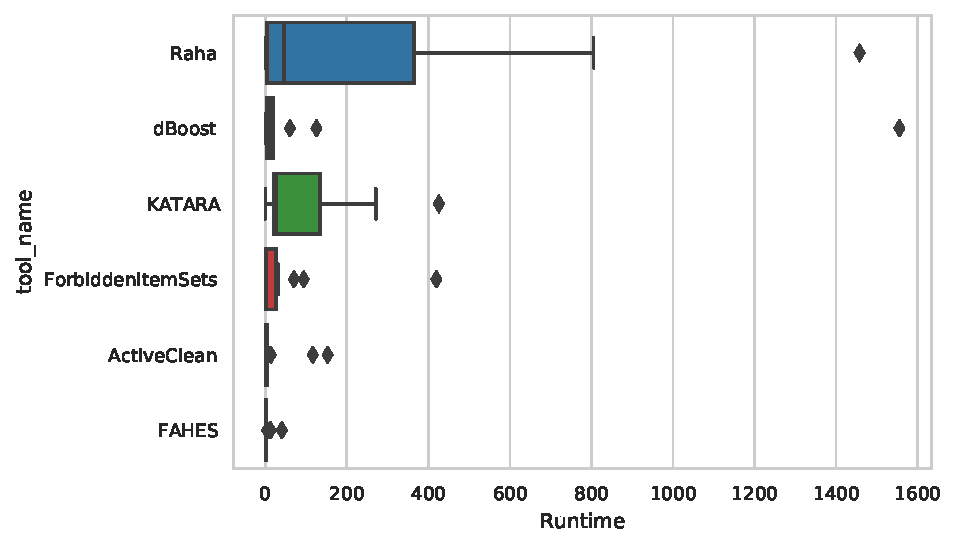
\includegraphics[width=\linewidth]{thesis/Figures/RQ1/RuntimeBoxplot.pdf}
    \end{adjustbox}
    \caption{Boxplot of the runtime in seconds for the best tool results}
    \label{fig:runtime_boxplot}
\end{figure}


% \paragraph{No human interaction} In the previous section, it has been shown that Raha performs best out of the 6 implemented tools. But, Raha is depending on user labeling. This means that the end-user of this error detection tool should be able to differentiate errors from the ground truth. If such a domain expert is not available, strategies without human interaction could be of interest. In \autoref{tab:empirical_results_no_human}, the same aggregated best (highest F1-score) performance scores for each tool per dataset are shown. The ActiveClean implementation does not have a configuration without human interaction. Raha does, but the best performing strategies were the ones that simply marked all cells as errors. Concluding from this table, it can be said that if there is not a user who can do the labeling for the domain of that dataset, dBoost will be the best solution to use.

% \begin{table}
% \centering
% \caption{|Precision Recall F1-score| for tool as column \& dataset as row \textbf{without human interaction}}
% \label{tab:empirical_results_no_human}
% \begin{adjustbox}{center}
% \begin{tabular}{llllll}
% \toprule
% {} & FAHES & ForbiddenItemSets & KATARA & Raha & dBoost \\
% \midrule
%  & \textbf{\space\space\space P \space\space\space\space R \space\space\space F1} & \textbf{\space\space\space P \space\space\space\space R \space\space\space F1} & \textbf{\space\space\space P \space\space\space\space R \space\space\space F1} & \textbf{\space\space\space P \space\space\space\space R \space\space\space F1} & \textbf{\space\space\space P \space\space\space\space R \space\space\space F1} \\
% airbnb & \textbf{0.54} 0.01 0.02 & 0.13 0.29 0.18 & Other error & Other error & 0.23 \textbf{0.38} \textbf{0.28} \\
% beers & \textbf{0.83} 0.02 0.04 & 0.34 0.30 0.32 & 0.14 0.26 0.18 & 0.16 \textbf{1.00} 0.28 & 0.68 0.55 \textbf{0.61} \\
% eeg & 0.00 0.00 0.00 & 0.02 0.26 0.04 & 0.00 0.00 0.00 & Other error & \textbf{0.13} \textbf{1.00} \textbf{0.23} \\
% flights & 0.23 0.01 0.02 & 0.56 0.16 0.24 & 0.09 0.09 0.09 & 0.30 \textbf{1.00} 0.46 & \textbf{0.94} 0.59 \textbf{0.72} \\
% hospital & 0.02 0.09 0.04 & 0.01 0.06 0.02 & \textbf{0.08} 0.37 \textbf{0.13} & 0.03 \textbf{1.00} 0.05 & 0.03 0.43 0.06 \\
% marketing & 0.24 0.01 0.01 & 0.25 0.46 0.33 & 0.21 0.32 0.25 & Other error & \textbf{0.34} \textbf{0.67} \textbf{0.45} \\
% movie & 0.00 0.00 0.00 & 0.31 0.08 0.13 & \textbf{0.43} 0.43 0.43 & Other error & 0.37 \textbf{1.00} \textbf{0.54} \\
% movies & 0.01 0.10 0.02 & 0.01 0.06 0.01 & \textbf{0.02} 0.16 \textbf{0.03} & 0.01 \textbf{1.00} 0.02 & 0.01 0.09 0.03 \\
% rayyan & 0.07 0.04 0.05 & Other error & 0.01 0.02 0.01 & 0.09 \textbf{1.00} 0.16 & \textbf{0.22} 0.77 \textbf{0.34} \\
% restaurant & 0.00 0.00 0.00 & 0.01 0.07 0.01 & 0.00 0.13 0.01 & 0.00 \textbf{1.00} 0.01 & \textbf{0.03} 0.03 \textbf{0.03} \\
% restaurants & \textbf{0.00} 0.07 \textbf{0.01} & Other error & 0.00 0.22 0.00 & 0.00 \textbf{1.00} 0.00 & 0.00 0.08 0.00 \\
% toy & 0.00 0.00 0.00 & 0.00 0.00 0.00 & 0.21 0.75 0.33 & 0.22 \textbf{1.00} 0.36 & \textbf{0.33} 0.75 \textbf{0.50} \\
% university & 0.00 0.00 0.00 & Other error & 0.06 0.29 0.10 & 0.03 \textbf{1.00} 0.05 & \textbf{0.32} \textbf{1.00} \textbf{0.49} \\
% uscensus & 0.01 0.18 0.02 & 0.02 0.26 0.04 & 0.00 0.00 0.00 & Other error & \textbf{0.41} \textbf{1.00} \textbf{0.58} \\
% \bottomrule
% \end{tabular}
% \end{adjustbox}
% \end{table}

% What if the best tool has 0.75 human expertise?
\subsection{Human accuracy influence}
If a user is willing and able to actively label cells during error detection, there still remains the question of how accurate those labels are. To show the implications of lesser accurate labeling, all the configuration of Raha were executed again, but the human interactions were simulated to be only 75\% accurate, instead of 100\%. The results are shown in \autoref{tab:raha_empirical}, with the fully accurate labeling on the left side, and the 75\% accuracy on the rights side. Immediately can be seen that tool is highly dependent on human accuracy. Only for 1 out of the 14 datasets, the tool randomly performed better with lower labeling accuracy according to the F1-score, then it did with full accuracy, due to the randomness in Raha. Nevertheless, precision-wise, for none of the datasets, the less accurate experiments produced better results than the fully accurate strategies. A user of interactive error detection tools should take this into account when deciding for an error detection tool. Solutions like repeated labeling by users could maybe mitigate the risk (as examples have shown by \cite{Sheng2008-gk}).

\begin{table}
\centering
\caption{|Precision Recall F1| for Raha with different human labeling accuracy (best scores in bold)}
\label{tab:raha_empirical}
\begin{tabular}{lll}
\toprule
{} & Raha 100\% & Raha 75\% \\
\midrule
 & \textbf{\space\space\space P \space\space\space\space R \space\space\space F1} & \textbf{\space\space\space P \space\space\space\space R \space\space\space F1} \\
airbnb & \textbf{0.42} 0.13 0.20 & 0.19 \textbf{0.36} \textbf{0.25} \\
beers & \textbf{0.97} 0.69 \textbf{0.80} & 0.70 \textbf{0.81} 0.75 \\
eeg & \textbf{0.56} \textbf{0.71} \textbf{0.63} & 0.10 0.44 0.16 \\
flights & \textbf{0.90} \textbf{0.83} \textbf{0.86} & 0.60 0.73 0.66 \\
hospital & \textbf{0.98} \textbf{0.57} \textbf{0.72} & 0.09 0.54 0.15 \\
marketing & \textbf{0.50} 0.32 \textbf{0.39} & 0.30 \textbf{0.47} 0.37 \\
movie & \textbf{0.47} 0.64 \textbf{0.54} & 0.41 \textbf{0.71} 0.52 \\
movies & \textbf{0.72} \textbf{0.76} \textbf{0.74} & 0.11 0.35 0.17 \\
rayyan & \textbf{0.86} 0.84 \textbf{0.85} & 0.71 \textbf{0.84} 0.77 \\
restaurant & \textbf{0.14} 0.11 \textbf{0.12} & 0.01 \textbf{0.58} 0.03 \\
restaurants & \textbf{0.00} \textbf{1.00} \textbf{0.00} & 0.00 0.00 0.00 \\
toy & \textbf{0.22} \textbf{1.00} \textbf{0.36} & Other error \\
university & \textbf{0.99} \textbf{0.91} \textbf{0.95} & 0.25 0.78 0.38 \\
uscensus & \textbf{1.00} \textbf{1.00} \textbf{1.00} & 0.05 0.64 0.09 \\
\bottomrule
\end{tabular}
\end{table}

\subsection{Results by error type}
In the following subsections, a more detailed review of results for the empirical study will be given. Where the previous sections would discuss overall performance, this section separates each error type for analysis, covering only overlapping tools that supposedly can detect such error types and datasets that contain these error types.

\subsubsection{Rule violations}
To start off, rule violations will be discussed. All the selected error detection tools have capabilities of detecting rule violations of some sort. Rule violations are also the most common error type occurring in datasets. All datasets except \verb|EEG|, \verb|Hospital| and \verb|Restaurants| contain errors detectable by rule violations. 
Because all tools and almost all datasets contain these error types, the general findings from \autoref{subsec:empirical_overall_results} apply to this specific error type. 

% \begin{table}[H]
% \centering
% \caption{Rule violations - |Precision Recall F1-score| for tool as column \& dataset as row}
% \begin{adjustbox}{center}
% \begin{tabular}{lllllll}
% \toprule
% {} & FAHES & KATARA & Raha & ActiveClean & dBoost & ForbiddenItemSets \\
% \midrule
%  & \textbf{\space\space\space P \space\space\space\space R \space\space\space F1} & \textbf{\space\space\space P \space\space\space\space R \space\space\space F1} & \textbf{\space\space\space P \space\space\space\space R \space\space\space F1} & \textbf{\space\space\space P \space\space\space\space R \space\space\space F1} & \textbf{\space\space\space P \space\space\space\space R \space\space\space F1} & \textbf{\space\space\space P \space\space\space\space R \space\space\space F1} \\
% university & 0.00 0.00 0.00 & 0.06 0.29 0.10 & \textbf{0.99} 0.91 \textbf{0.95} & 0.03 0.09 0.04 & 0.32 \textbf{1.00} 0.49 & Other error \\
% movies & 0.01 0.10 0.02 & 0.02 0.16 0.03 & \textbf{0.72} \textbf{0.76} \textbf{0.74} & 0.02 0.00 0.01 & 0.01 0.09 0.03 & 0.01 0.06 0.01 \\
% restaurant & 0.00 0.00 0.00 & 0.00 0.13 0.01 & \textbf{0.14} 0.11 \textbf{0.12} & 0.01 \textbf{0.83} 0.02 & 0.03 0.03 0.03 & 0.01 0.07 0.01 \\
% beers & 0.83 0.02 0.04 & 0.14 0.26 0.18 & \textbf{0.97} 0.69 \textbf{0.80} & 0.16 \textbf{1.00} 0.28 & 0.68 0.55 0.61 & 0.34 0.30 0.32 \\
% uscensus & 0.01 0.18 0.02 & 0.00 0.00 0.00 & \textbf{1.00} \textbf{1.00} \textbf{1.00} & 0.02 0.00 0.00 & 0.41 \textbf{1.00} 0.58 & 0.02 0.26 0.04 \\
% flights & 0.23 0.01 0.02 & 0.09 0.09 0.09 & 0.90 0.83 \textbf{0.86} & 0.30 \textbf{0.98} 0.46 & \textbf{0.94} 0.59 0.72 & 0.56 0.16 0.24 \\
% movie & 0.00 0.00 0.00 & 0.43 0.43 0.43 & \textbf{0.47} 0.64 \textbf{0.54} & 0.37 \textbf{1.00} 0.54 & 0.37 \textbf{1.00} 0.54 & 0.31 0.08 0.13 \\
% toy & 0.00 0.00 0.00 & 0.21 0.75 0.33 & 0.22 \textbf{1.00} 0.36 & Other error & \textbf{0.33} 0.75 \textbf{0.50} & 0.00 0.00 0.00 \\
% airbnb & \textbf{0.54} 0.01 0.02 & Other error & 0.42 0.13 0.20 & 0.15 \textbf{1.00} 0.26 & 0.23 0.38 \textbf{0.28} & 0.13 0.29 0.18 \\
% marketing & 0.24 0.01 0.01 & 0.21 0.32 0.25 & \textbf{0.50} 0.32 0.39 & 0.25 0.36 0.30 & 0.34 \textbf{0.67} \textbf{0.45} & 0.25 0.46 0.33 \\
% rayyan & 0.07 0.04 0.05 & 0.01 0.02 0.01 & \textbf{0.86} 0.84 \textbf{0.85} & 0.09 \textbf{1.00} 0.16 & 0.22 0.77 0.34 & Other error \\
% \bottomrule
% \end{tabular}
% \end{adjustbox}
% \end{table}


\subsubsection{Pattern violations}
The two tools capable of detecting pattern violations are Raha and dBoost. Both error detection tools are capable of detecting multiple error types, but it is clear that Raha outperforms dBoost. In most datasets that have pattern violation errors, will also contain rule violations. dBoost has limited multicolumn error detection (with the Gaussian mixed models), compared to Raha, which could lead to the lower results. However, for highly structured datasets like \verb|Flights|, that contained information like time and flight number, dBoost is capable of finding outliers in the patterns from these columns.
Because Raha has underlying pattern detection tools it learns from (dBoost implementation) and the aid of a human expert, it is more capable of capturing all errors holistically, including pattern violations.

\begin{table}[H]
\centering
\caption{Pattern violations - |Precision Recall F1| for tool as column \& dataset as row (best scores in bold)}
\begin{adjustbox}{center}
\begin{tabular}{lll}
\toprule
{} & Raha & dBoost \\
\midrule
 & \textbf{\space\space\space P \space\space\space\space R \space\space\space F1} & \textbf{\space\space\space P \space\space\space\space R \space\space\space F1} \\
beers & \textbf{0.97} \textbf{0.69} \textbf{0.80} & 0.68 0.55 0.61 \\
flights & 0.90 \textbf{0.83} \textbf{0.86} & \textbf{0.94} 0.59 0.72 \\
hospital & \textbf{0.98} \textbf{0.57} \textbf{0.72} & 0.03 0.43 0.06 \\
movies & \textbf{0.72} \textbf{0.76} \textbf{0.74} & 0.01 0.09 0.03 \\
rayyan & \textbf{0.86} \textbf{0.84} \textbf{0.85} & 0.22 0.77 0.34 \\
restaurant & \textbf{0.14} \textbf{0.11} \textbf{0.12} & 0.03 0.03 0.03 \\
restaurants & 0.00 \textbf{1.00} \textbf{0.00} & \textbf{0.00} 0.08 0.00 \\
\bottomrule
\end{tabular}
\end{adjustbox}
\end{table}

One of the surprising results is those of the \verb|Restaurants| dataset. This dataset has a data quality of 99.9\%, meaning that less than 0.1\% of the data cells are errors. Rounded, this will result in a precision of 0.00 for Raha, but with a recall of 1.00. This means that the best error detection job it could do, was simply marking all the values as erroneous, leading to this rather uncommon precision and recall tuple of 0.00 and 1.00. 

\subsubsection{Outliers}
The errors that can be detected as outliers are detectable by again Raha and dBoost. The only two datasets containing classical outliers are \verb|Airbnb| and \verb|EEG|. In terms of F1-score, dBoost outperforms for \verb|Airbnb|. For dBoost, there are configurations that achieve higher precision, at the cost of lower recall. This means that for detecting outliers, if dBoost is configured with more conservative thresholds for outlier detection, it could be of great value in an automated error detection pipeline. 

\begin{table}[H]
\centering
\caption{Outliers - |Precision Recall F1| for tool as column \& dataset as row (best scores in bold)}
\begin{adjustbox}{center}
\begin{tabular}{lll}
\toprule
{} & Raha & dBoost \\
\midrule
 & \textbf{\space\space\space P \space\space\space\space R \space\space\space F1} & \textbf{\space\space\space P \space\space\space\space R \space\space\space F1} \\
airbnb & \textbf{0.42} 0.13 0.20 & 0.23 \textbf{0.38} \textbf{0.28} \\
eeg & \textbf{0.56} 0.71 \textbf{0.63} & 0.13 \textbf{1.00} 0.23 \\
\bottomrule
\end{tabular}
\end{adjustbox}

\end{table}

\subsubsection{Duplicates}
The two tools capturing complete information about a row are ActiveClean and Raha, making it possible for these two tools to detect duplicates that are errors. \verb|Airbnb| and \verb|Movie| are the datasets containing duplicates. ActiveClean has a higher F1-score for \verb|Airbnb|, but always lower precision. The precision of ActiveClean is equal to the portion of errors in those datasets, showing that ActiveClean simply labels all values as erroneous, which is not a valuable error detection result. 

\begin{table}[H]
\centering
\caption{Duplicates - |Precision Recall F1| for tool as column \& dataset as row (best scores in bold)}
\begin{adjustbox}{center}
\begin{tabular}{lll}
\toprule
{} & ActiveClean & Raha \\
\midrule
 & \textbf{\space\space\space P \space\space\space\space R \space\space\space F1} & \textbf{\space\space\space P \space\space\space\space R \space\space\space F1} \\
airbnb & 0.15 \textbf{1.00} \textbf{0.26} & \textbf{0.42} 0.13 0.20 \\
movie & 0.37 \textbf{1.00} 0.54 & \textbf{0.47} 0.64 \textbf{0.54} \\
\bottomrule
\end{tabular}
\end{adjustbox}
\end{table}

\subsection{Evaluation}
\label{subsec:evaluation_empirical_study_results}
The results from the empirical study have one clear outcome. Raha has the highest performance scores, at the cost of human expertise while detecting errors and the highest execution times. 
Raha outperforms or scores equally for grouped experiments based on error types. This could be because of the following:
\begin{itemize}
    \item Raha is capable to "capture" more complex characteristics due to the human in the loop.
    \item Only two datasets contained a single error type. All others contained a mixture of error types.
\end{itemize}

In other studies, like done by \cite{Abedjan2016-jc}, the researchers included data cleaning tools with predefined cleaning rules or functional dependencies. This research aims to find completely automated or active learning error detection tools with no extra human configuration. Without user-defined function or rules as input to the error detection tools, automated cleaning tools will perform less on these heterogeneous datasets. With an active cleaning tool like Raha, these rules can be implicitly be transferred by actively labeling error clusters.

In the empirical study, there was no tool included for designated duplicate detection. Although datasets in the empirical study contained duplicates, there was no specific tool to detect duplicates row-wise explicitly. The study might benefit from having an error type-specific error detection tool for each error type, to give a complete overview of their workings on real-life datasets.

% Rerun stochastic error detection tools -> How to train or score estimators? 
Also, ActiveClean and Raha are partially based on random sampling for labeling errors actively during cleaning. Different samples could lead to different results for the same configuration and dataset. Running strategies is a time-consuming process, so repeated experiments were not feasible for this stage of the research. This means that, depending on the (partially) random sampling, the same configuration could perform differently. This should be taken into account in further research. 

~\\To summarize, the current state of the art was represented by 6 different error detection tools, namely: ActiveClean, dBoost, FAHES, Forbidden Itemsets, KATARA and Raha. The performance of Raha, a human-interactive tool was the best according to the F1-measure, both overall as well as in the detailed analysis grouped on error types. In using Raha, there is a caveat, namely that the tool is highly dependent on the accuracy of the human labeling the errors in the active learning process. 